% !TEX root = ../main.tex

\chapter{规划器测试与实验}\label{chap:experiments}

\section{引言}\label{sec:intro_5}
本章对前文所设计的过驱动飞行器的6自由度规划器进行一系列实验。
\ref{sec:planner_performance}节对规划器的效果进行测试,
对比分析了使用欧拉角姿态表示法和使用四元数姿态表示法(以下简称欧拉角法和四元数法)两种情况下规划器的性能特点;
\ref{sec:simulation_experiments}节和\ref{sec:real_world_experiments}节分别令OmniHex的仿真模型和实物飞行器执行规划器给出的轨迹,
初步验证了本课题规划器的可行性。

\section{规划器效果测试}\label{sec:planner_performance}
本节通过在各种给定的环境中运行本课题开发的过驱动飞行器轨迹器来测试其效果,
并将结果使用Rviz\cite{kam2015rviz}等可视化工具进行展示。

测试过程中环境地图作为已知量,主要使用点云和八叉树两种表达形式,规划方式为全局规划。
重点关注输出轨迹的避障特性以及规划过程的计算效率。
未经特殊说明,本节实验的规划器参数设置如\tabref{tab:planner_parameter_setting}
计算过程中物理量均取其在国际单位制下的数值大小。

\begin{table}[htbp]
    \caption{实验中规划器的参数设置\label{tab:planner_parameter_setting}}
    \vspace{0.5em}\centering\wuhao
    \begin{tabular}{cc}
    \toprule[1.5pt]
    参数 & 取值\\
    \midrule[1pt]
    长方体尺寸 & (1.0m, 1.0m, 0.35m) \\
    RRT步长 & 0.5 \\ 
    RRT采样概率 & 0.9 \\
    初始轨迹中间点间距 & 3.0m \\
    $k_\rho$ & 100.0 \\
    $(v_{max}, W_v)$ & (0.8m$\cdot$ s$^{-1}$, 1$\times$10$^{4}$) \\
    $(a_{max}, W_a)$ & (5.0m$\cdot$ s$^{-2}$, 1$\times$10$^{4}$) \\
    $(\omega_{max}, W_\omega)$ & (0.8rad$\cdot$ s$^{-1}$, 1$\times$10$^{4}$) \\
    $W_c$ & 9$\times$10$^{4}$ \\
    \bottomrule[1.5pt]
    \end{tabular}
  \end{table}

\subsection{随机地图中的轨迹规划}\label{subsec:planning_in_random_map}
\begin{figure}[!ht]
    \setlength{\subfigcapskip}{-1bp}
    \centering
    \begin{minipage}{\textwidth}
  
    \centering
    \subfigure{\label{fig:random_map_overview}}\addtocounter{subfigure}{-2}
    \subfigure{\subfigure[随机地图概览]{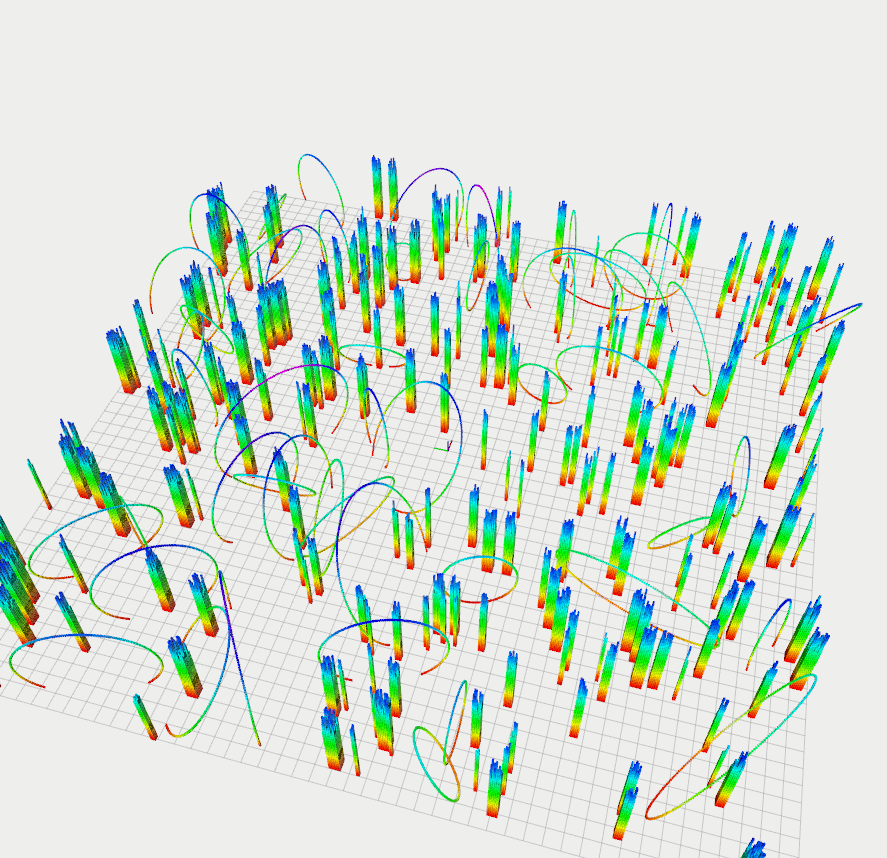
\includegraphics[width=0.3\textwidth]{random_map_overview.png}}}
    \hspace{0.2em}
    \subfigure{\label{fig:cylinder_obstacles}}\addtocounter{subfigure}{-2}
    \subfigure{\subfigure[柱形障碍物]{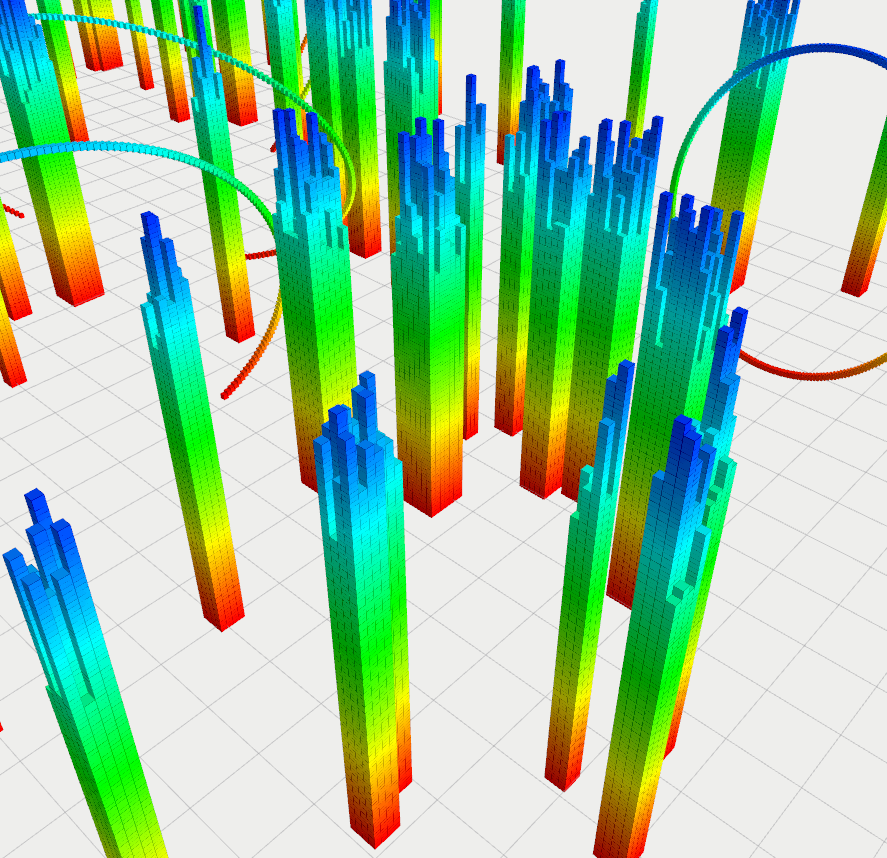
\includegraphics[width=0.3\textwidth]{cylinder_obstacles.png}}}
    \hspace{0.2em}
    \subfigure{\label{fig:circle_obstacles}}\addtocounter{subfigure}{-2}
    \subfigure{\subfigure[圆圈形障碍物]{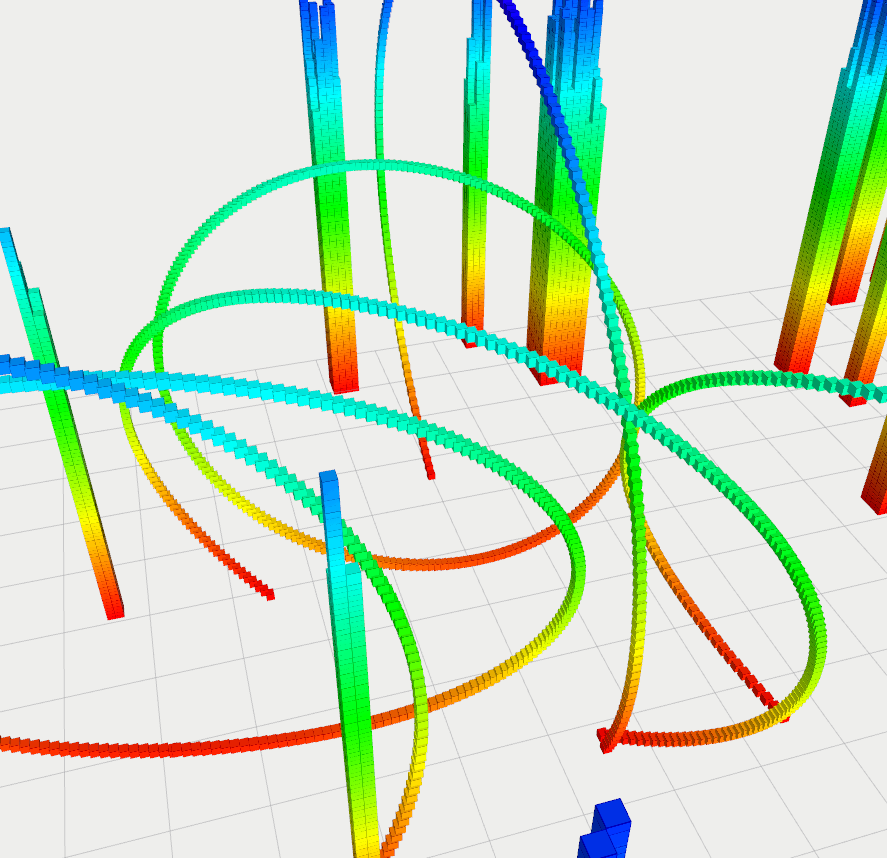
\includegraphics[width=0.3\textwidth]{circle_obstacles.png}}}
    
    \end{minipage}
    \caption{随机地图示意图}
    \label{fig:random_map}
  \end{figure}
本小节在使用现成随机地图生成程序生成的随机环境(如\figref{fig:random_map_overview}所示)中进行规划。
该程序可以根据人为指定的地图范围、障碍物数量即分辨率将障碍物随机布撒到环境中,并以点云的形式输出。
障碍物分为柱形(\figref{fig:cylinder_obstacles})和圆圈形(\figref{fig:circle_obstacles}),
二者的尺寸范围也可以人为设置

\figref{fig:random_map_planning}中分别展示了使用基于欧拉角和基于四元数两种姿态表示法在随机地图中规划出的轨迹,
轨迹多项式的次数为7(即$s=4$),
地图尺寸为50m$\times$50m,其中随机分布有300个柱形障碍物和30个圆圈形障碍物,
轨迹起始条件和终止条件中速度、加速度、加加速度以及姿态对应的RPY角均为0。

\begin{figure}[!ht]
    \setlength{\subfigcapskip}{-1bp}
    \centering
    \begin{minipage}{\textwidth}
  
    \centering
    \subfigure{\label{fig:random_map_planning_rpy}}\addtocounter{subfigure}{-2}
    \subfigure{\subfigure[基于欧拉角]{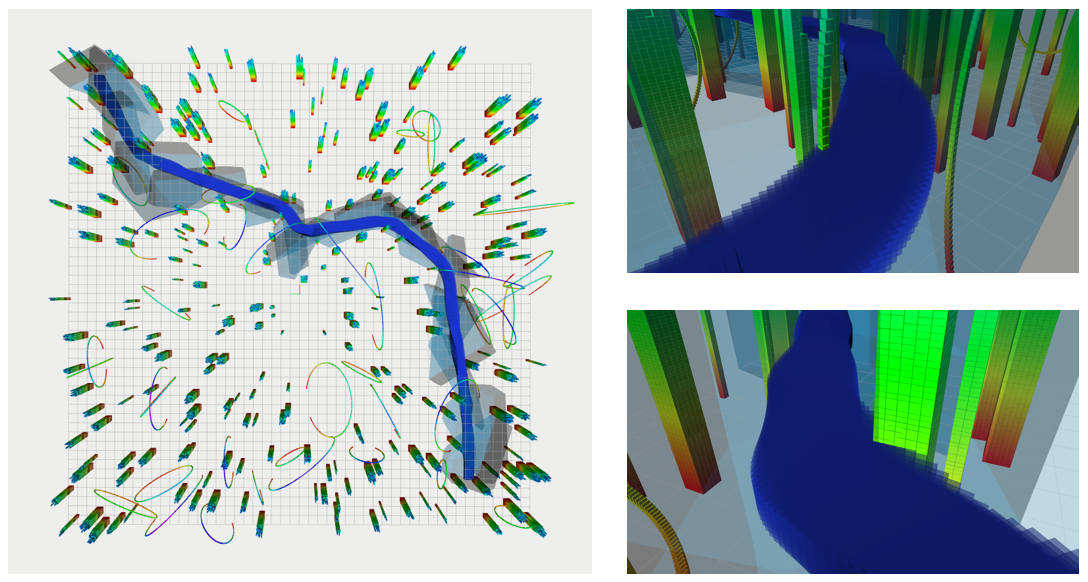
\includegraphics[width=0.88\textwidth]{random_map_rpy_planning.png}}}
    
    \subfigure{\label{fig:random_map_planning_quat}}\addtocounter{subfigure}{-2}
    \subfigure{\subfigure[基于四元数]{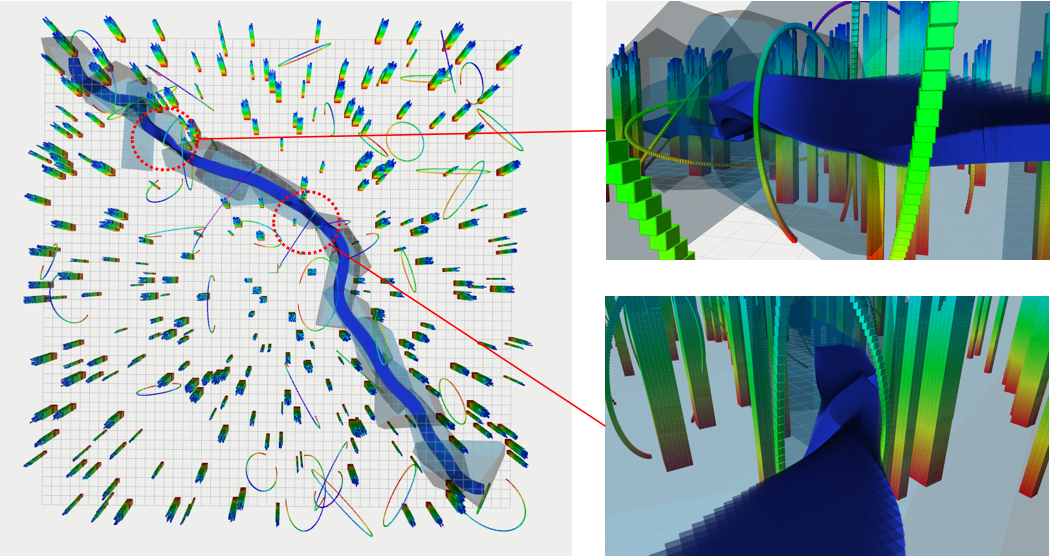
\includegraphics[width=0.88\textwidth]{random_map_quat_planning.png}}}
    
    \end{minipage}
    \caption{在随机地图中进行规划得到的轨迹及其局部细节}
    \label{fig:random_map_planning}
\end{figure}

\figref{fig:random_map_planning}中一系列半透明浅蓝色凸多面体为生成的飞行走廊,
而深蓝色带状物则是由近似表示飞行器形状的长方体组成轨迹可视化的6自由度轨迹。
可以看到,生成的轨迹均被成功约束在了安全飞行走廊内,且具有足够的平滑性。

如\figref{fig:dynamic_properties}所示分别画出了上述两条轨迹的动力学特性,
\figref{fig:dyn_prop_quat}和\figref{fig:dyn_prop_rpy}所展示的是整条轨迹中速率、加速率和角速率的变化,
红色虚线表示的是动力学限制$v_{max}$、$a_{max}$和$\omega_{max}$,
可见轨迹的动力学特性被有效地约束住了,
且在时间正则项的作用下,轨迹在大部分时间内都达到了所限制的最大速率。
\figref{fig:dyn_prop_3d_quat}和\figref{fig:dyn_prop_3d_rpy}所展示的则是速度、加速度和角速度向量的轨迹,
图中淡黄色的球所表示的则是$v_{max}$、$a_{max}$和$\omega_{max}$。

\begin{figure}[!ht]
    \setlength{\subfigcapskip}{-1bp}
    \centering
    \begin{minipage}{\textwidth}

    \centering
    \subfigure{\label{fig:dyn_prop_quat}}\addtocounter{subfigure}{-2}
    \subfigure{\subfigure[基于欧拉角法规划的轨迹动力学特性]{\includegraphics[width=0.47\textwidth]{random_map_rpy_2/dyn.png}}}
    \hspace{0.2em}
    \subfigure{\label{fig:dyn_prop_3d_quat}}\addtocounter{subfigure}{-2}
    \subfigure{\subfigure[基于欧拉角法规划的轨迹动力学特性(3D)]{\includegraphics[width=0.47\textwidth]{random_map_rpy_2/dyn_3d.png}}}

    \centering
    \subfigure{\label{fig:dyn_prop_rpy}}\addtocounter{subfigure}{-2}
    \subfigure{\subfigure[基于四元数法规划的轨迹动力学特性]{\includegraphics[width=0.47\textwidth]{random_map_quat_4/dyn.png}}}
    \hspace{0.2em}
    \subfigure{\label{fig:dyn_prop_3d_rpy}}\addtocounter{subfigure}{-2}
    \subfigure{\subfigure[基于四元数法规划的轨迹动力学特性(3D)]{\includegraphics[width=0.47\textwidth]{random_map_quat_4/dyn_3d.png}}}
    
    \end{minipage}
    \caption{所得轨迹的动力学特性示意图}
    \label{fig:dynamic_properties}
\end{figure}

上述两种规划结果的前后端相关数据如\tabref{tab:data_of_2_scenarios_in_random_map}所示,其中$t_{\text{opt}}$表示整个轨迹优化过程的耗时。
表中数据与\figref{fig:random_map_planning}表现出了两种不同规划方式各自的典型特征,
\begin{enumerate}
    \renewcommand{\labelenumi}{(\theenumi)}
    \item 此场景下基于欧拉角的方法轨迹优化速度通常比基于四元数的方法更快;
    \item 相较基于欧拉角的方法而言,基于四元数的方法对狭小的空间和障碍无更为“敏感”:
    基于四元数的方法规划出的轨迹在穿过狭小的空间或者经过靠近障碍物的地方时更倾向于倾斜姿态来避免碰撞,并且常常会牺牲轨迹的局部平滑度来达到避障的目的;
    而基于欧拉角的方法显得更为“懒惰”,常常靠近障碍物处也不会利用姿态控制来规避障碍物,所以轨迹上经常会有刮蹭发生,
    其表现出倾向于轨迹平滑度而不是避障性能的特点。
\end{enumerate}

\begin{table}[htbp]
    \caption{随机地图规划两种方式前后端相关数据\label{tab:data_of_2_scenarios_in_random_map}}
    \vspace{0.5em}\centering\wuhao
    \begin{tabular}{ccccc}
    \toprule[1.5pt]
    姿态规划方式 & RRT耗时(秒) & 生成SFC耗时 & SFC凸多面体数 & $t_{\text{opt}}$(秒)\\
    \midrule[1pt]
    四元数 & 0.206 & 0.951 & 14 & 10.799 \\
    欧拉角 & 0.431 & 0.898 & 20 & 4.609 \\
    \bottomrule[1.5pt]
    \end{tabular}
\end{table}

首先分析优化效率的不同,考虑到两种规划方式的差异最终都体现到了罚函数$I_\Sigma$值与梯度的计算上,
\tabref{tab:analysis_of_efficiency_in_random_map_scenario}进一步给出了相关数据作对比。
其中$t_{\text{col}}$、$t_{\text{dyn}}$及$t_{\text{pen}}$分别表示单次计算碰撞惩罚项、动力学约束惩罚项以及整个罚函数的耗时。
可见在单次计算罚函数的耗时以及拟牛顿法迭代次数上四元数法均比欧拉角法更有优势,
但是最后的总优化时间却比欧拉角法要慢得多,
这说明在线搜索阶段四元数法的迭代次数远多于欧拉角法的,
于是可以推断四元数法目标函数的数值特性不利于线搜索。
至于欧拉角法以更快的速度优化出的轨迹对障碍物敏感程度不够的原因,
推测是由于欧拉角法的目标函数存在较多的局部最小值。

\begin{table}[htbp]
    \caption{随机地图规划两种方式的效率分析\label{tab:analysis_of_efficiency_in_random_map_scenario}}
    \vspace{0.5em}\centering\wuhao
    \begin{tabular}{ccccccc}
    \toprule[1.5pt]
    姿态规划方式 & $t_{\text{col}}$(毫秒) & $t_{\text{dyn}}$(毫秒)& $t_{\text{pen}}$(毫秒)& L-BFGS迭代次数 & $t_{\text{opt}}$(秒)\\
    \midrule[1pt]
    四元数 & 1.564 & 0.307 & 1.877 & 30 & 10.799 \\
    欧拉角 & 1.891 & 0.261 & 2.159 & 1788 & 4.609 \\
    \bottomrule[1.5pt]
    \end{tabular}
\end{table}

为更细致地研究两种不同的姿态规划方法在安全性和快速性,
本课题进一步设计了定量实验。

为衡量安全性,首先约定规划成功的定义:
\begin{definition}
    \equref{equ:final_unconstrained_optimization_problem}表示的6自由度轨迹优化问题在时间间隔$\Delta t$下称为是成功的,当且仅当以下条件得到满足:
    \begin{enumerate}
        \renewcommand{\labelenumi}{(\theenumi)}
        \item 优化过程不因函数值出现NaN或无穷大等原因而中断;
        \item 在最后优化出的轨迹上以$\Delta t$为间隔取点,所有点对应的$SE(3)$状态经有效性检测的结果均为有效状态。
    \end{enumerate}
\end{definition}

据此设计以下定量实验来估计不同姿态规划方法及参数在不同障碍物密度下的成功率:
固定地图中存在障碍物分布的部分的尺寸,以及轨迹起始条件和终止条件,
在不同的障碍物数量下分别进行多次(100次)规划,每次规划前均重新生成随机地图,
记录不同障碍物数量下的成功率来粗略衡量对应规划方法和参数条件的安全性能。

这里选取了相同规划器参数条件下使用四元数法和欧拉角法的两种规划方式作对照,
并且猜想欧拉角法对与障碍物的不敏感性可能是因为碰撞惩罚项相较控制代价而言不足以主导目标函数最小化过程,
故又添加了具有更大碰撞惩罚权重$W_c$的欧拉角法作为对照组,
以此探究增大$W_c$对欧拉角法安全性能的改进程度。
实验结果如\figref{fig:success_rates}所示:

\begin{figure}[ht]
    \centering
    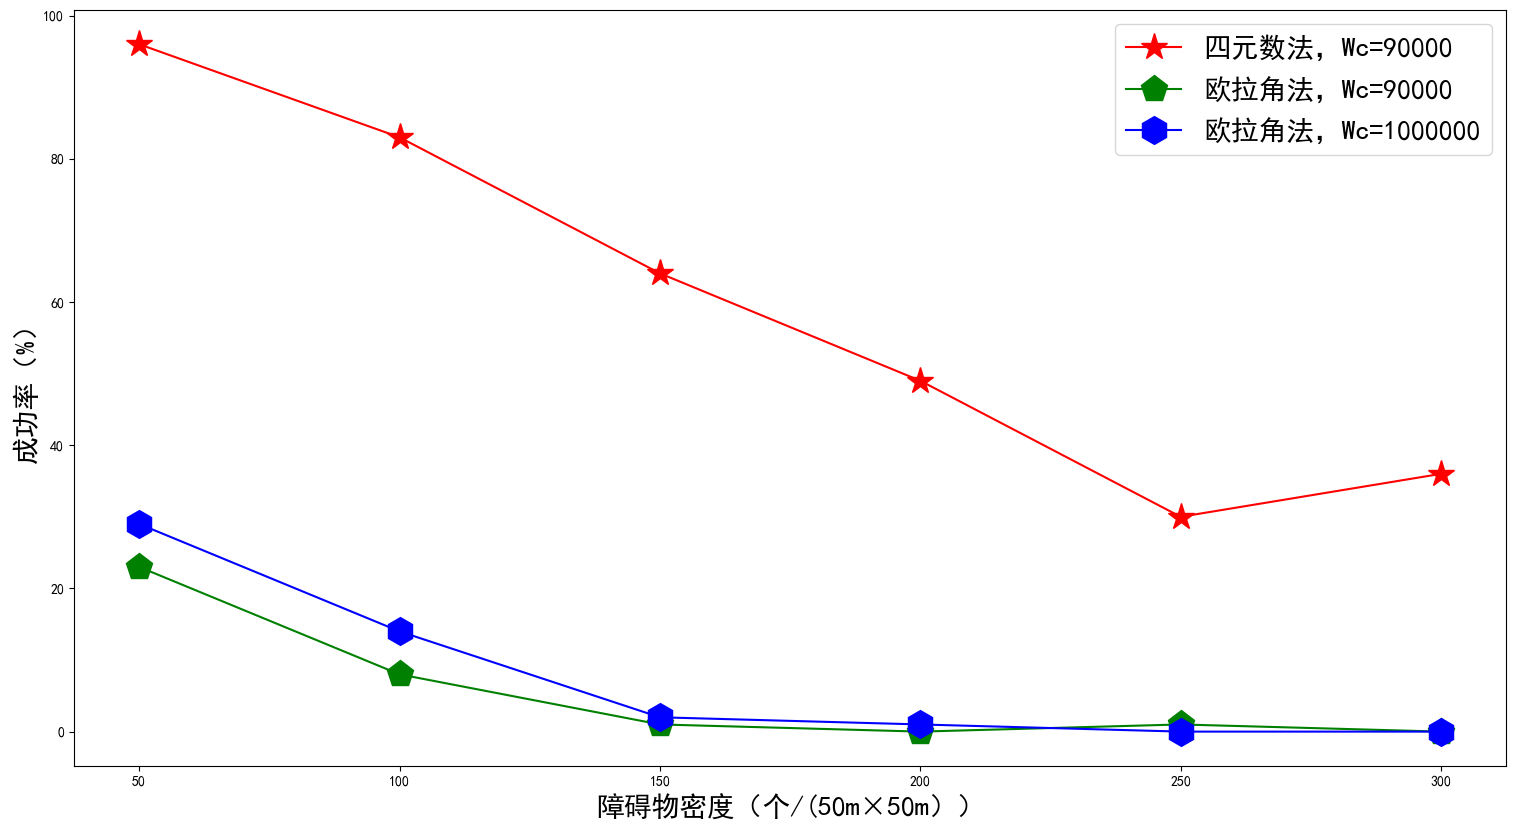
\includegraphics[width = 0.86\textwidth]{success_rates.png}
    \caption{不同障碍物密度下的规划成功率}
    \label{fig:success_rates}
\end{figure}

发现在五种障碍物密度下,四元数法的成功率都要远高于欧拉角法,且提高欧拉角法的$W_c$对其成功率的改善十分微弱。

不过由于飞行走廊的存在,不论是欧拉角法还是四元数法,即使轨迹存在碰撞,绝大多数情况下也都是些“小擦小碰”,
实际应用中可以通过对飞行器尺寸采取更保守的近似,或者提高飞行器的抗轻微碰撞的能力来弥补。
上述成功的定义稍显苛刻,如果在对无碰撞要求不那么高的情况下,也可以使用欧拉角法来加快求解速度。

\begin{table}[htbp]
    \caption{两种规划方式平均每段轨迹的平均优化时间\label{tab:mean_opt_time_per_segment}}
    \vspace{0.5em}\centering\wuhao
    \begin{tabular}{ccccccc}
    \toprule[1.5pt]
    姿态规划方式 &  $({{t_{\text{opt}}}}/M)$均值(秒)\\
    \midrule[1pt]
    四元数 & 0.388 \\
    欧拉角 & 0.106 \\
    \bottomrule[1.5pt]
    \end{tabular}
\end{table}

在计算时间方面,由于优化过程单次迭代的时间复杂度为线性的$O(M)$,
即单次耗时近似与轨迹段数$M$成正比(不同的飞行走廊凸多面体之间的差异带来的影响可忽略不计),
故同种规划方式的优化总时间$t_{\text{opt}}$也应与$M$近似成正比,
因此平均每段轨迹的优化时间$t_{\text{opt}}/M$能更准确地反映出规划效率。
由上述成功率实验中测出的欧拉角法与四元数法平均结果如\tabref{tab:mean_opt_time_per_segment}所示,
可见在计算时间方面欧拉角法确实更胜一筹。

\subsection{狭窄空间中的轨迹规划}\label{subsec:planning_in_narrow_env}
本小节测试所开发的规划器在狭窄空间中的避障性能。
规划器需要为过驱动飞行器规划出穿越一条长约6m、宽约0.3m的狭长通道的无碰撞6自由度轨迹,
这里将长方体厚度$l_z$取为0.3m,实际场合中这应该是一个比飞行器最大厚度稍大的值。

\begin{figure}[!ht]
    \setlength{\subfigcapskip}{-1bp}
    \centering
    \begin{minipage}{\textwidth}

    \centering
    \subfigure{\label{fig:narrow_passage_rpy_1}}\addtocounter{subfigure}{-2}
    \subfigure{\subfigure[欧拉角法1]{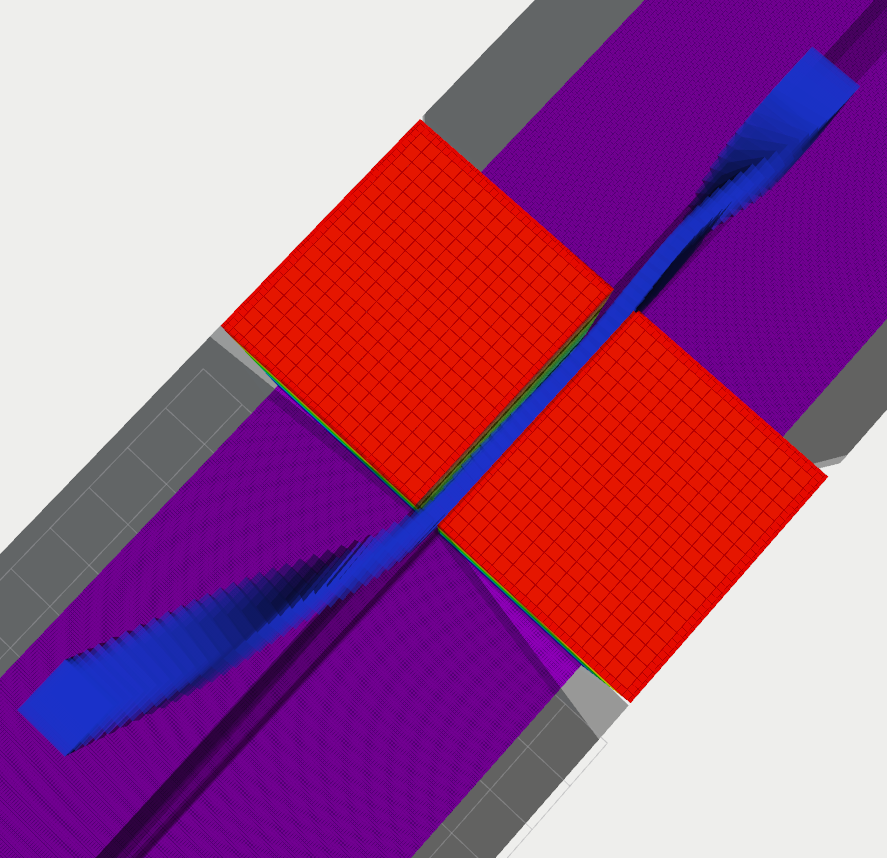
\includegraphics[width=0.22\textwidth]{narrow_passage_rpy_1.png}}}
    \hspace{0.2em}
    \subfigure{\label{fig:narrow_passage_rpy_2}}\addtocounter{subfigure}{-2}
    \subfigure{\subfigure[欧拉角法2]{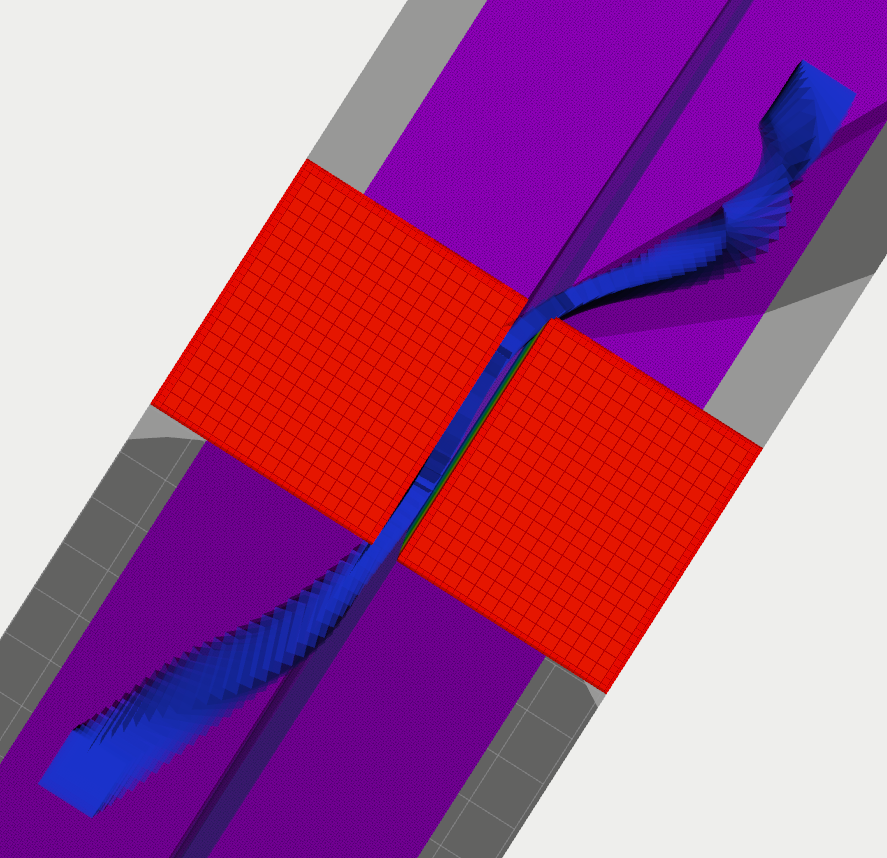
\includegraphics[width=0.22\textwidth]{narrow_passage_rpy_2.png}}}
    \hspace{0.2em}
    \centering
    \subfigure{\label{fig:narrow_passage_quat_1}}\addtocounter{subfigure}{-2}
    \subfigure{\subfigure[四元数法1]{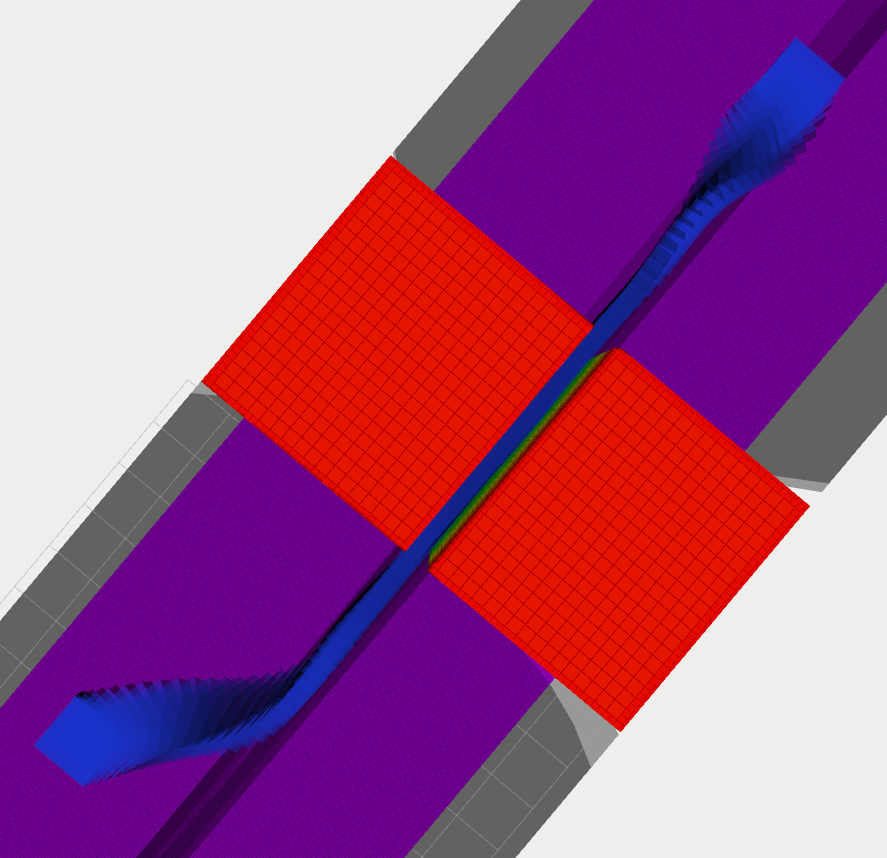
\includegraphics[width=0.22\textwidth]{narrow_passage_quat_1.png}}}
    \hspace{0.2em}
    \subfigure{\label{fig:narrow_passage_quat_2}}\addtocounter{subfigure}{-2}
    \subfigure{\subfigure[四元数法2]{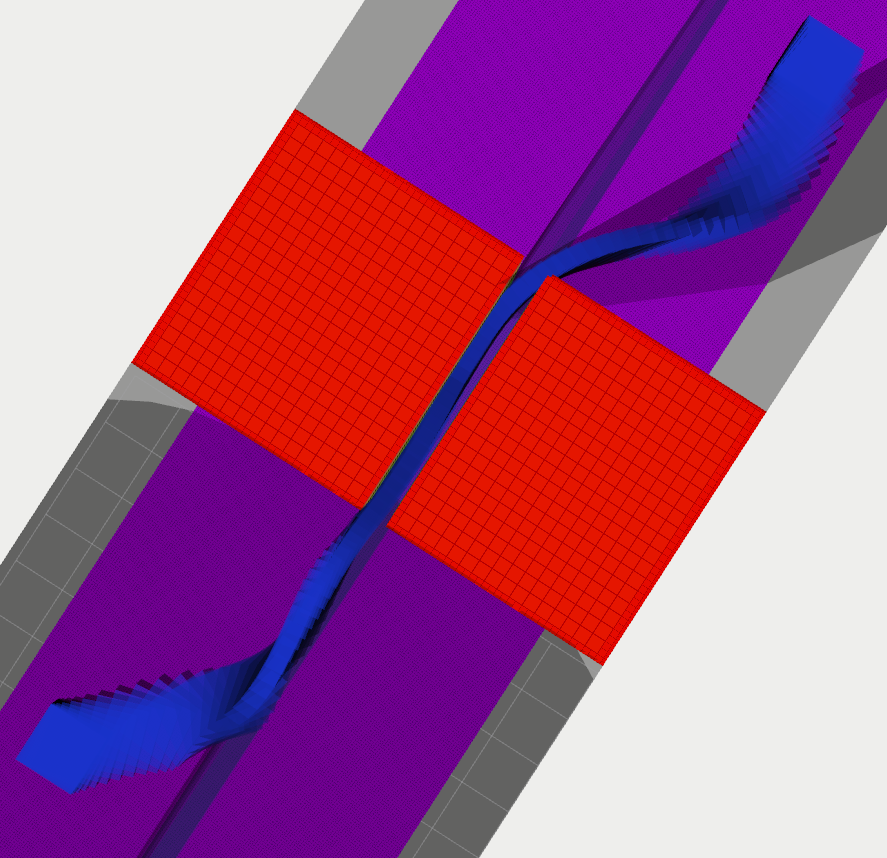
\includegraphics[width=0.22\textwidth]{narrow_passage_quat_2.png}}}
    
    \end{minipage}
    \caption{在狭长通道中所规划出的6自由度轨迹}
    \label{fig:planning_in_narrow_passage}
\end{figure}
\begin{figure}[ht]
    \setlength{\subfigcapskip}{-1bp}
    \centering
    \begin{minipage}{\textwidth}

    \centering
    \subfigure{\label{fig:narrow_passage_rpy_detail_1}}\addtocounter{subfigure}{-2}
    \subfigure{\subfigure[欧拉角法1]{\includegraphics[width=0.4\textwidth]{narrow_passage_rpy_1/detail_1.png}}}
    \hspace{0.2em}
    \subfigure{\label{fig:narrow_passage_rpy_detail_2}}\addtocounter{subfigure}{-2}
    \subfigure{\subfigure[欧拉角法2]{\includegraphics[width=0.4\textwidth]{narrow_passage_rpy_1/detail_2.png}}}
    
    \subfigure{\label{fig:narrow_passage_quat_detail_2}}\addtocounter{subfigure}{-2}
    \subfigure{\subfigure[四元数法1]{\includegraphics[width=0.4\textwidth]{narrow_passage_quat_1/detail_1.png}}}
    \hspace{0.2em}
    \subfigure{\label{fig:narrow_passage_quat_detail_2}}\addtocounter{subfigure}{-2}
    \subfigure{\subfigure[四元数法2]{\includegraphics[width=0.4\textwidth]{narrow_passage_quat_1/detail_2.png}}}
    
    \end{minipage}
    \caption{狭长通道中6自由度轨迹局部细节}
    \label{fig:details_of_planning_in_narrow_passage}
\end{figure}

本小节同样分别使用四元数和欧拉角两种姿态规划方法做了实验,
其结果可视化如\figref{fig:planning_in_narrow_passage}所示,
由于在起点和终点被狭窄通道隔开的情况下RRT很难找到可行解,
且本小节重点关注只在后端部分进行的轨迹优化算法的表现,
\figref{fig:planning_in_narrow_passage}中所得结果的前端路径采用A*算法来得到。
不论是哪种方法均能令轨迹倾斜姿态从而规避障碍物(\figref{fig:details_of_planning_in_narrow_passage}),
但在途中所示的场景下四元数法的表现比欧拉角法要稳定,
其优化时间基本在1秒以内,
而欧拉角法的优化时间在1秒以内到数十秒不等。


如\figref{fig:planning_in_complex_env}所示展示了四元数法在一个更复杂的环境中规划出的轨迹,
该轨迹成功通过灵活改变姿态安全穿越了连续的狭小区域。
初始路径使用RRT搜索出来,该场景优化时间基本稳定在10秒上下。

\begin{figure}[!ht]
    \setlength{\subfigcapskip}{-1bp}
    \centering
    \begin{minipage}{\textwidth}
  
    \centering
    \subfigure{\label{fig:complex_env_and_traj_overview}}\addtocounter{subfigure}{-2}
    \subfigure{\subfigure[环境地图与规划出的轨迹]{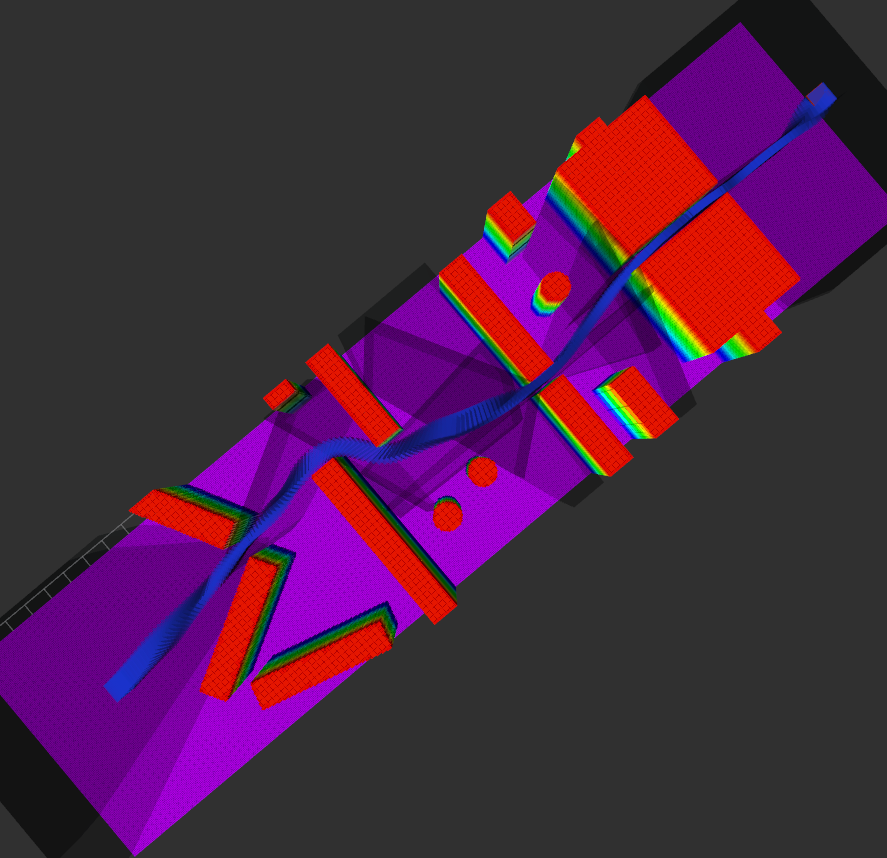
\includegraphics[width=0.3\textwidth]{sfc_and_traj.png}}}
    \hspace{0.2em}
    \subfigure{\label{fig:complex_env_and_traj_detail_1}}\addtocounter{subfigure}{-2}
    \subfigure{\subfigure[局部细节1]{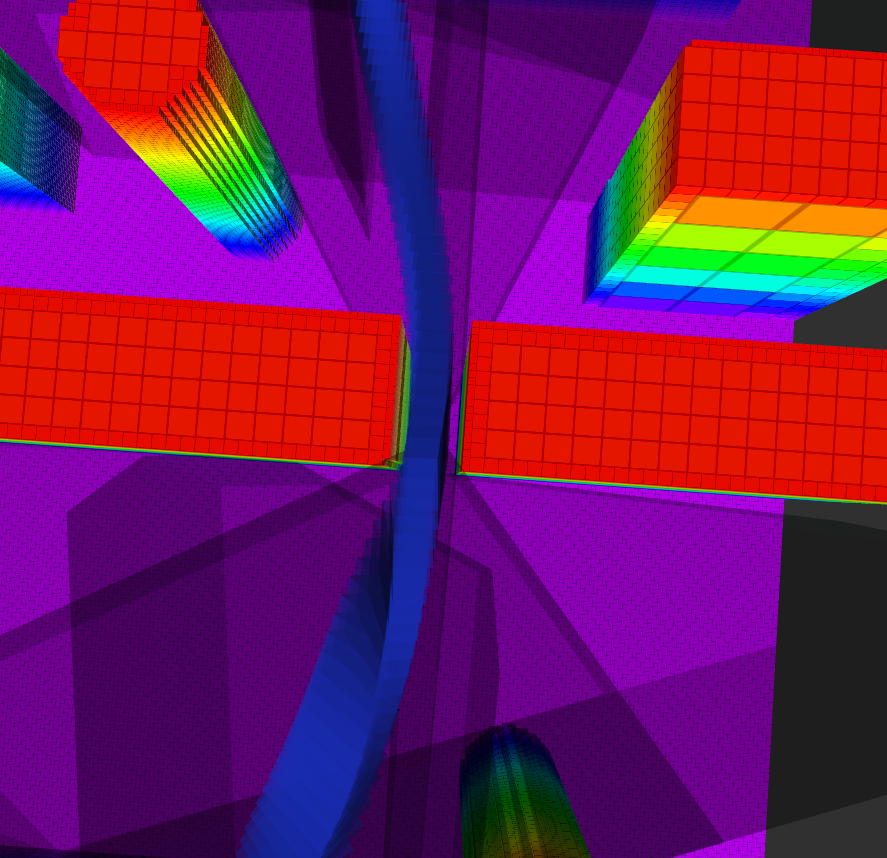
\includegraphics[width=0.3\textwidth]{traj_detail_2.png}}}
    \hspace{0.2em}
    \subfigure{\label{fig:complex_env_and_traj_detail_2}}\addtocounter{subfigure}{-2}
    \subfigure{\subfigure[局部细节2]{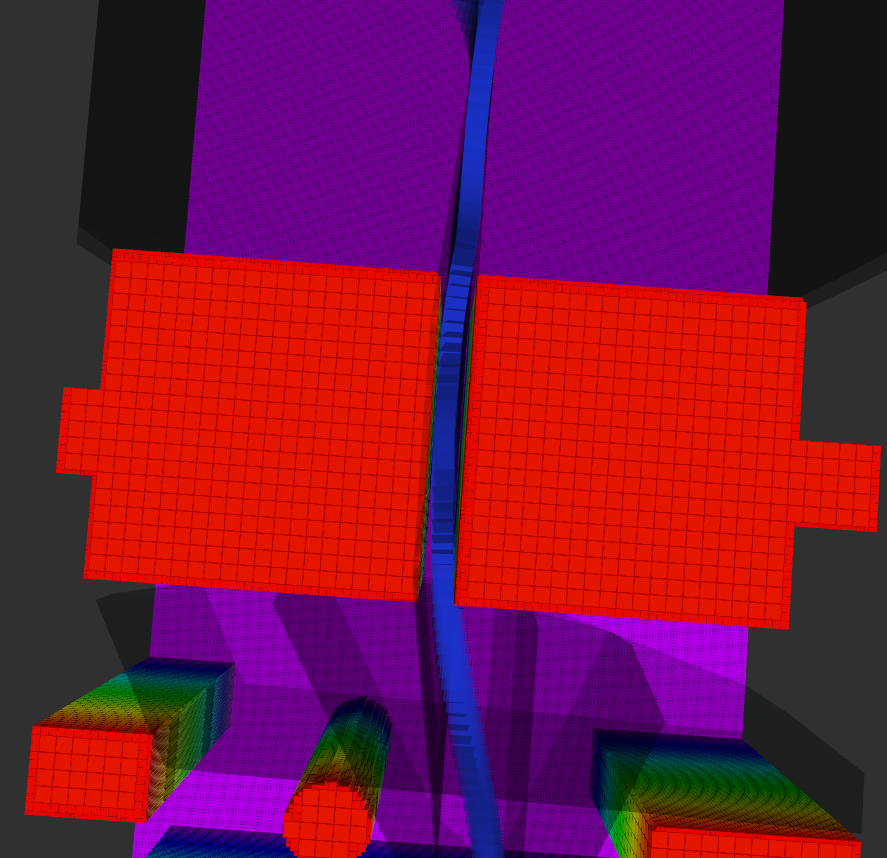
\includegraphics[width=0.3\textwidth]{traj_detail_3.png}}}
    
    \end{minipage}
    \caption{复杂环境中的规划}
    \label{fig:planning_in_complex_env}
  \end{figure}

欧拉角法也能成功在\figref{fig:planning_in_complex_env}所示的环境中规划出类似的轨迹,
但其有不小的几率在最后的狭长通道中产生“拧麻花”现象(\figref{fig:problem_when_using_rpy}),
导致轨迹与障碍物发生较为严重的碰撞

\begin{figure}[ht]
    \centering
    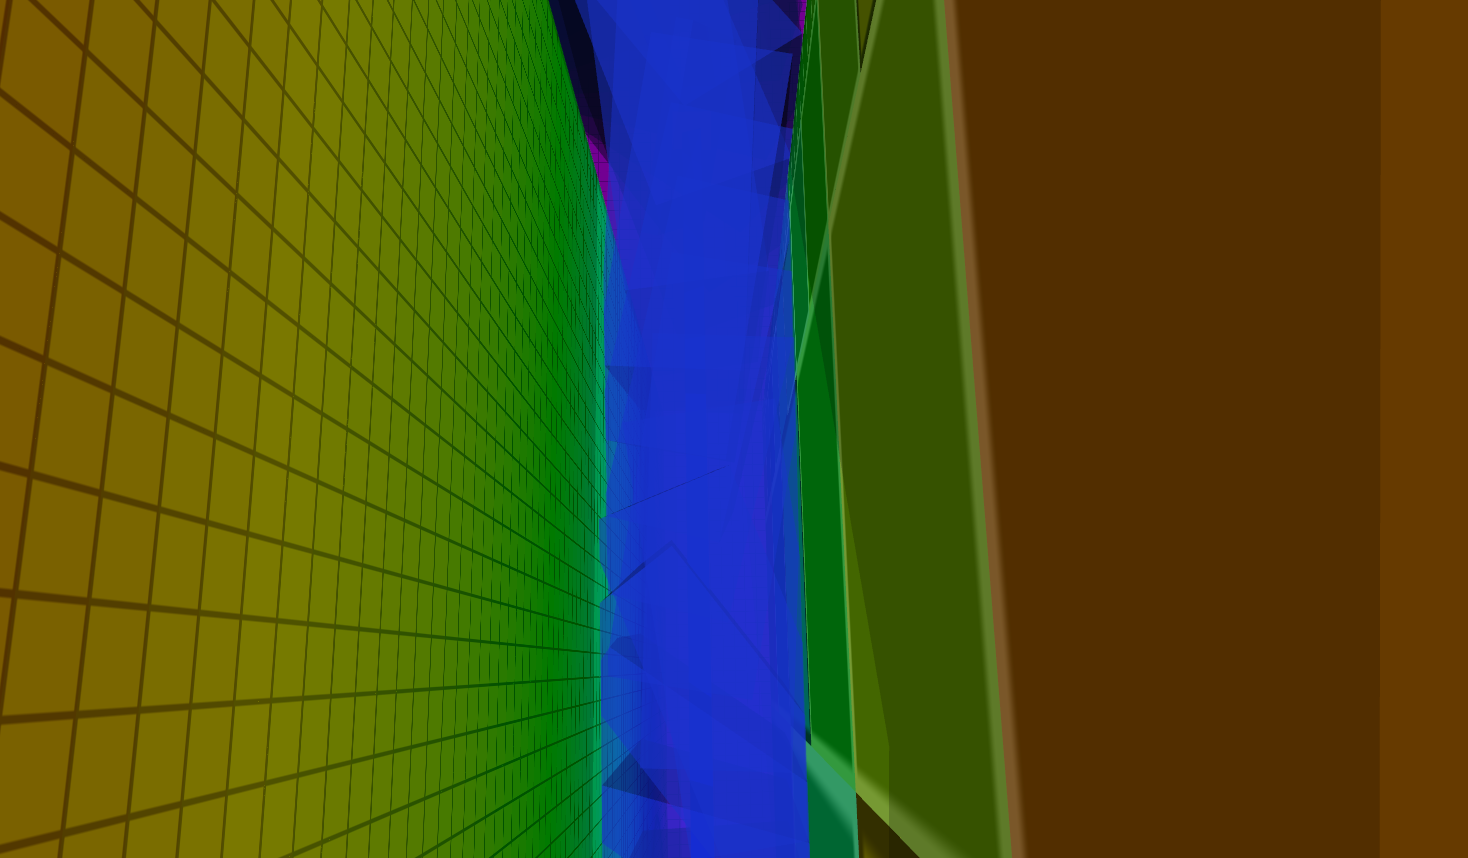
\includegraphics[width = 0.8\textwidth]{problem_when_using_rpy.png}
    \caption{欧拉角法的“拧麻花现象”}
    \label{fig:problem_when_using_rpy}
\end{figure}

% \begin{table}[htbp]
%     \caption{两种姿态规划方式在穿越狭窄缝隙的场景下的一些数据对比\label{tab:comparison_in_narrow_gap_scenario}}
%     \vspace{0.5em}\centering\wuhao
%     \begin{tabular}{cccccc}
%     \toprule[1.5pt]
%     姿态规划方式 & $t_{\text{col}}$(毫秒) & $t_{\text{dyn}}$(毫秒)& $t_{\text{pen}}$(毫秒)& L-BFGS迭代次数 & $t_{\text{opt}}$(秒)\\
%     \midrule[1pt]
%     四元数 & 0.182 & 0.055 & 0.242 & 90 & 0.838 \\
%     欧拉角 & 0.230 & 0.052 & 0.286 & 2244 & 0.842\\
%     \bottomrule[1.5pt]
%     \end{tabular}
% \end{table}

\subsection{规划器性能总结}
本节测试并对比了基于欧拉角法和基于四元数法的规划器的性能。
欧拉角法的主要优势为计算速度通常较快,且规划出的轨迹较为平滑,
缺点是对障碍物不够敏感,规划出的轨迹经常发生擦碰,
且在极端环境中有一定几率会触发严重碰撞;
四元数法的主要优势为对障碍物敏感,
常常会为规避碰撞而牺牲一点平滑度,
规划出的轨迹安全性较高,
其缺点除了平滑度稍差外,就是计算时间稍长。

综上所述,二者各有优劣。
如果追求轨迹的安全性能而不那么在意计算速度,可以选择四元数法;
如果环境不那么极端(像\figref{fig:planning_in_complex_env}中那样),
且飞行器对抗碰撞干扰能力较强,对微小擦碰不那么在意的情况下,可以选择欧拉角法。

几何约束轨迹优化算法所有流程的时间复杂度均为线性复杂度$O(M)$,
而本课题的是通过串行的方式实现的轨迹优化算法,且实现代码并不一定是最优的,
所以考虑到还有代码优化与并行计算等手段并未使用,
本课题所开发的规划算法在计算效率上应当还有不少提升空间。
如此看来,相对于欧拉角法来说四元数法的潜能应该更大,
本章后续实验均采用四元数法来为过驱动飞行器规划轨迹。

\section{仿真避障测试}\label{sec:simulation_experiments}
本节将基于Gazebo仿真环境与PX4飞行控制软件进行仿真避障实验,
以初步验证本课题所设计的规划算法的可行性。
\begin{figure}[!ht]
    \centering
    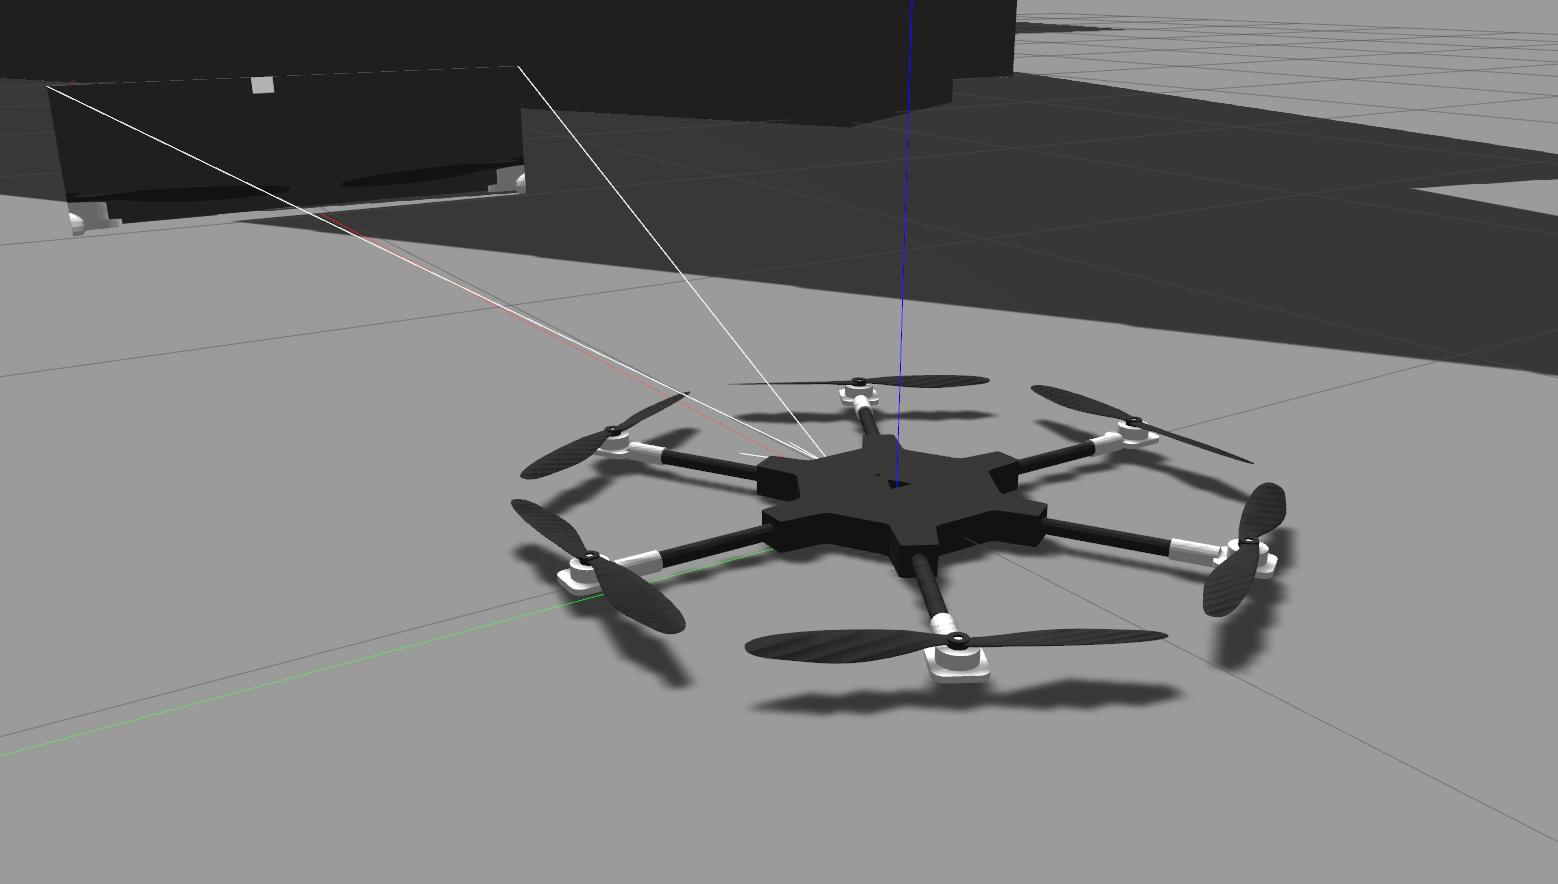
\includegraphics[width = 0.8\textwidth]{simplified_simulation_model.jpg}
    \caption{简化版OmniHex仿真模型}
    \label{fig:simplified_simulation_model}
\end{figure}
\subsection{真值地图的生成}
本课题不为OmniHex的仿真模型和实物配备感知系统,而是将环境信息作为已知量,
因此要进行仿真实验,就需要从Gazebo仿真环境中生成真值地图。

本课题采用的方案是采用的方案是编写 Gazebo 插件,该插件在仿真启动时被加载,
此时插件可以通过调用 Gazebo提供的 API 来获取仿真环境信息。
按照给定的范围和分辨率检查仿真空间中一系列离散点的碰撞情况,得到环境的点云信息,
然后利用 PCL 库和 Octomap 库进行处理可分别得到点云真值地图和八叉树真值地图。

如\figref{fig:planning_in_narrow_passage}和\figref{fig:planning_in_complex_env}中的地图都是用这种方法从Gazebo环境中直接生成的。

\subsection{仿真效果展示}
由于本小节主要演示过驱动飞行器OmniHex在复杂环境中的避障飞行,
且为了减轻仿真系统的负担、加快仿真流畅度,
本课题的仿真实验采用如\figref{fig:simplified_simulation_model}所示仅保留机身中心板和倾转旋翼单元的简化版模型,
采用PID算法进行轨迹跟踪控制。

首先我们规划出一条穿越狭缝的轨迹让飞行器在仿真中执行, 
展示了规划出的轨迹以及仿真中飞行器的实际轨迹,
实际轨迹采用视频逐帧叠加的方式合成在一张图片里,
从图中可以清晰地看到飞行器准确地执行了轨迹,
灵活地倾斜自己的姿态以适应狭缝中的空间并流畅地完成穿越。

\begin{figure}[!ht]
    \setlength{\subfigcapskip}{-1bp}
    \centering
    \begin{minipage}{\textwidth}
  
    \centering
    \subfigure{\label{fig:sim_narrow_gap_traj}}\addtocounter{subfigure}{-2}
    \subfigure{\subfigure[规划出的轨迹]{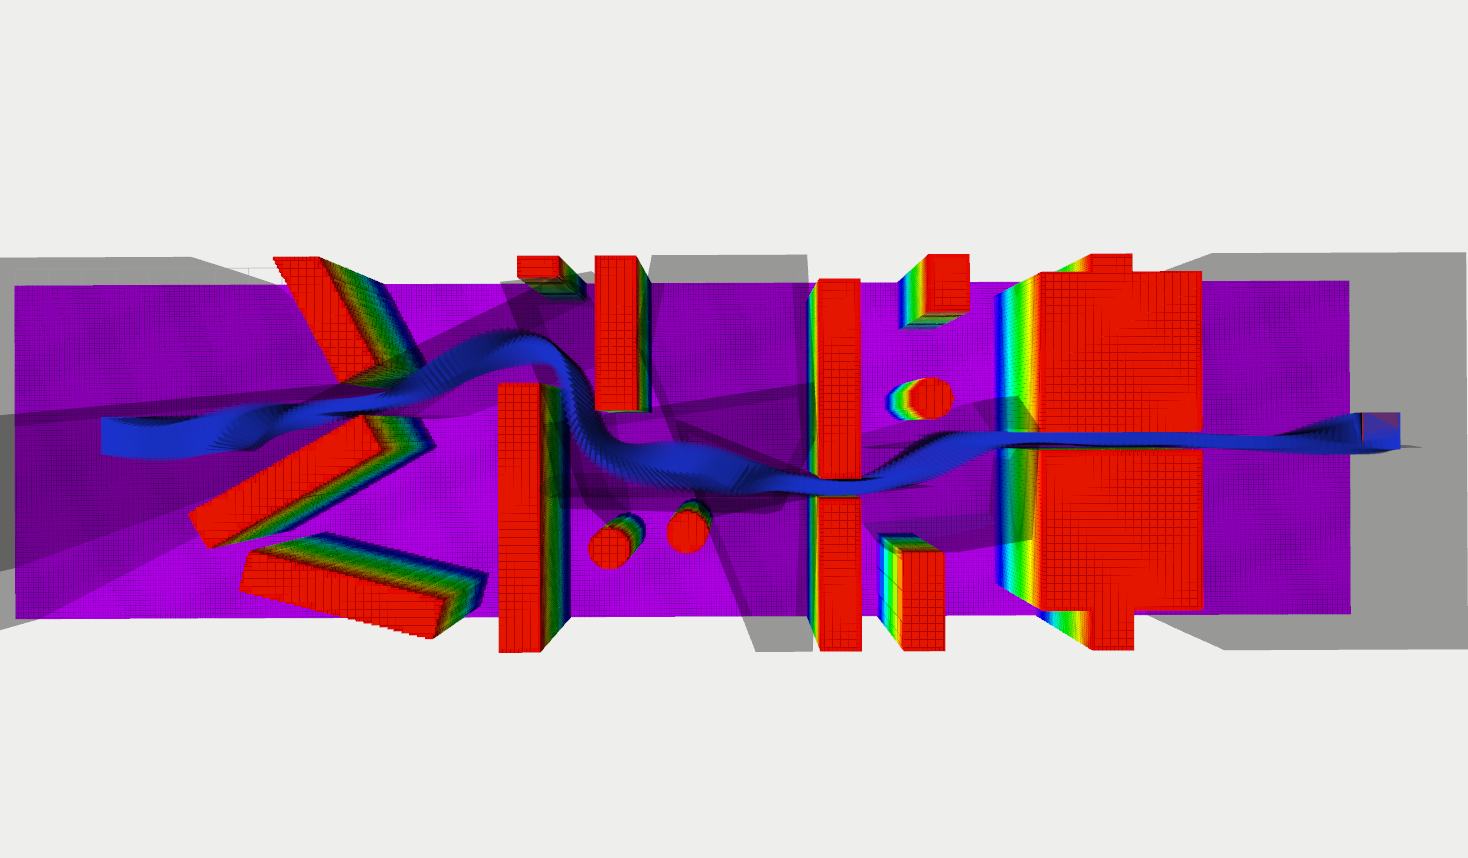
\includegraphics[width=0.45\textwidth]{narrow_gap_sim_1/traj.png}}}
    \hspace{0.2em}
    \subfigure{\label{fig:sim_narrow_gap_actual}}\addtocounter{subfigure}{-2}
    \subfigure{\subfigure[仿真中实际执行的轨迹]{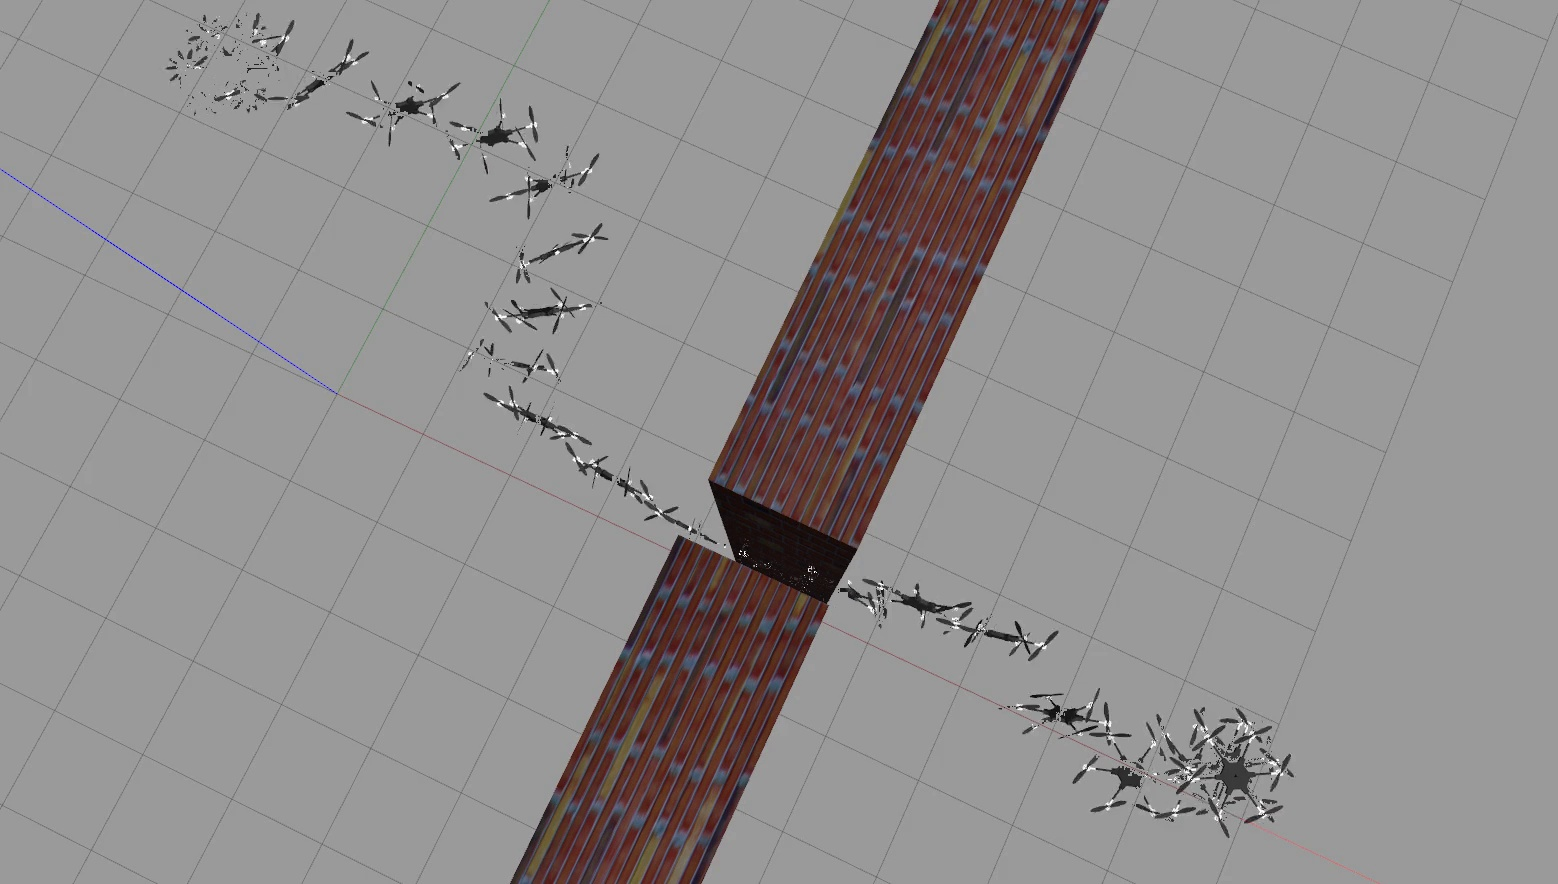
\includegraphics[width=0.45\textwidth]{narrow_gap_sim_1/out.jpg}}}
    
    \end{minipage}
    \caption{穿越夹缝仿真}
    \label{fig:narrow_gap_simulation}
  \end{figure}

如\figref{fig:complex_env_simulation}所示为仿真中飞行器执行规划器规划出的6自由度轨迹安全穿越更复杂环境的过程。
\begin{figure}[ht]
    \centering
    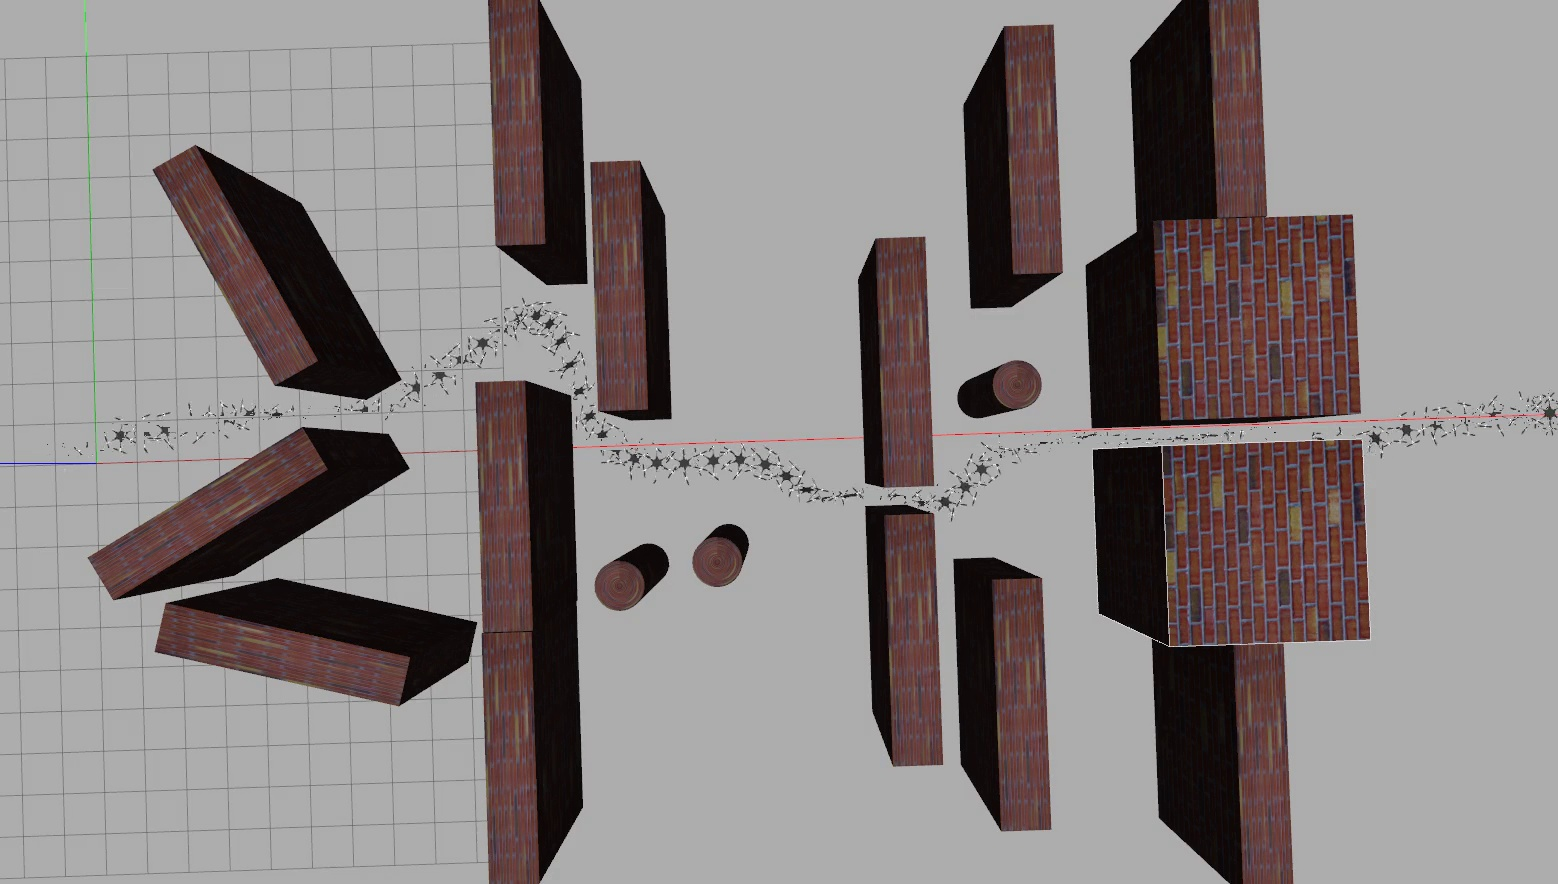
\includegraphics[width = 0.8\textwidth]{complex_env_simulation.jpg}
    \caption{复杂环境中的避障仿真}
    \label{fig:complex_env_simulation}
\end{figure}

\section{实物避障测试}\label{sec:real_world_experiments}
TODO
\section{本章小结}\label{sec:summary_5}
本章首先从安全性和快速性两方面对所设计的规划器进行性能测试,
对比分析了欧拉角法和四元数法两种方法的优势与短板;
随后在仿真环境和真实世界中让飞行器执行所规划出的轨迹,
初步验证了本文所提出的过驱动飞行器轨迹规划算法的可行性。
